\documentclass{article}
\usepackage{graphicx}
\usepackage{subfigure}

\title{Optimizador de resultados - QAOA}
\date{}

\begin{document}
\maketitle

Para mejorar los resultados de QAOA tras ejecutar el algoritmo.

\textbf{Idea: } Pasar el valor de la función de coste (\textit{cost(x)}) por algún tipo de hipérbola, para maximizar los resultados de bajo coste y minimizar los de alto.

La idea es dada un array de bits resultantes obtener $c' = \frac{1}{cost(bits)}*p$, donde \textit{p} es el número de ``counts'' obtenidas en la ejecución del algoritmo y también el eje \textit{y} de los histogramas mostrados.

\begin{figure}[htbp]
  \centering
  \subfigure[Antes de la ejecución]{
    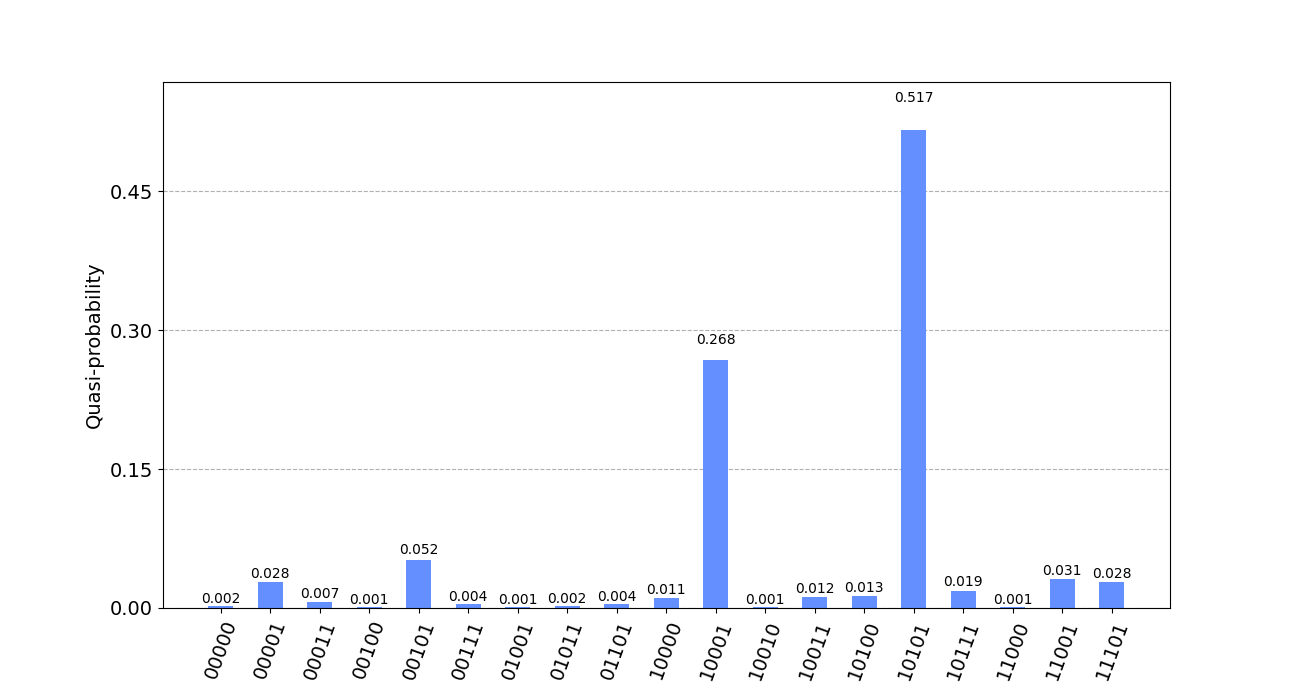
\includegraphics[width=0.47\textwidth]{caso_1_old}
  }
  \subfigure[Después de la ejecución]{
    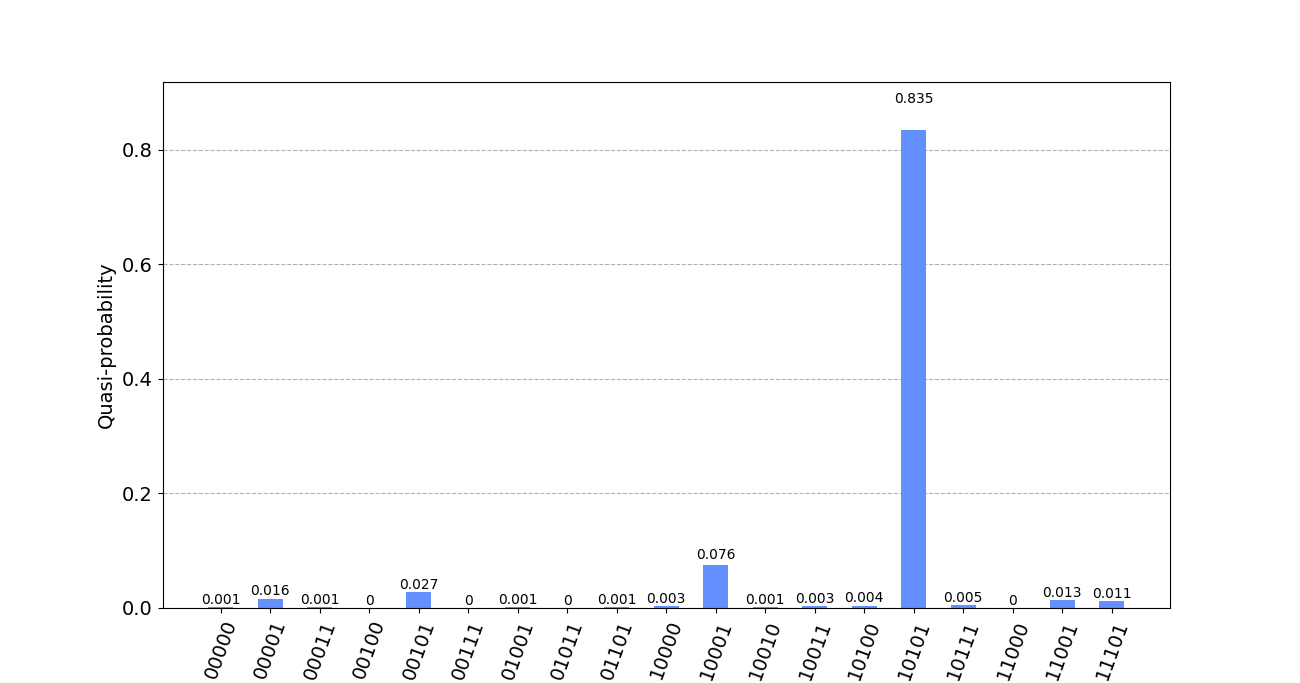
\includegraphics[width=0.47\textwidth]{caso_1_new}
  }
  \caption{Primer caso}
\end{figure}

\begin{figure}[htbp]
  \centering
  \subfigure[Antes de la ejecución]{
    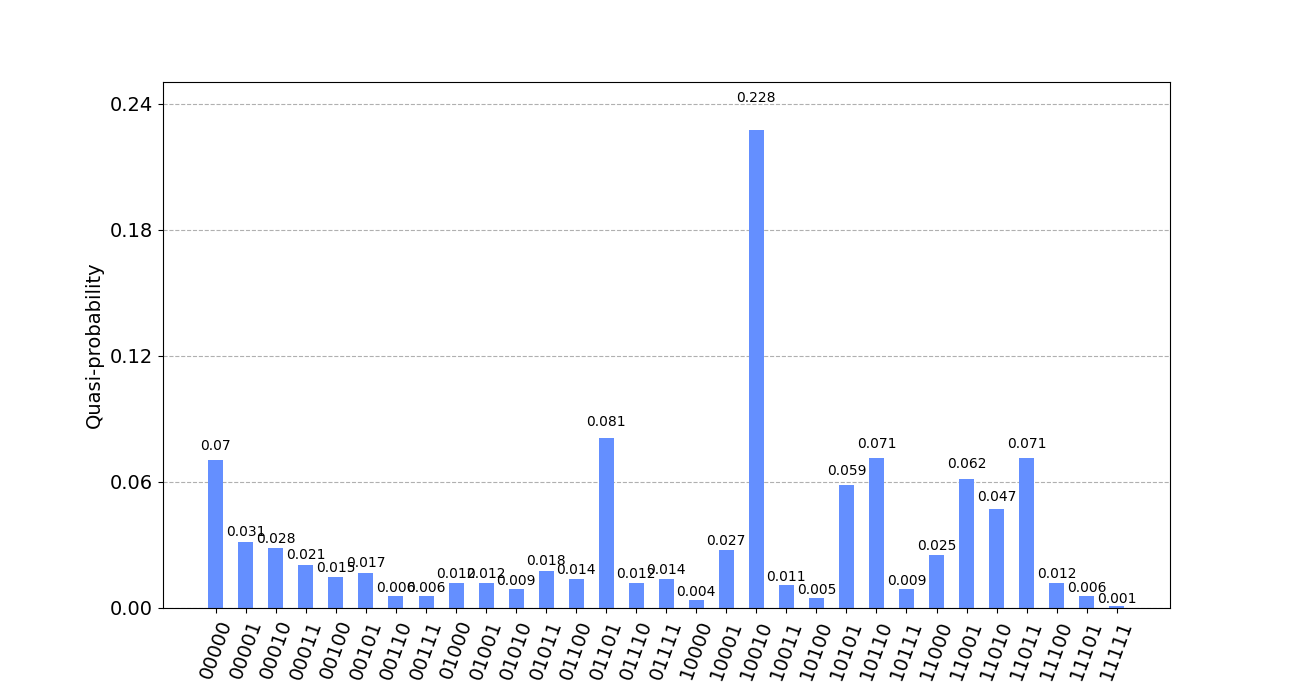
\includegraphics[width=0.47\textwidth]{caso_2_old}
  }
  \subfigure[Después de la ejecución]{
    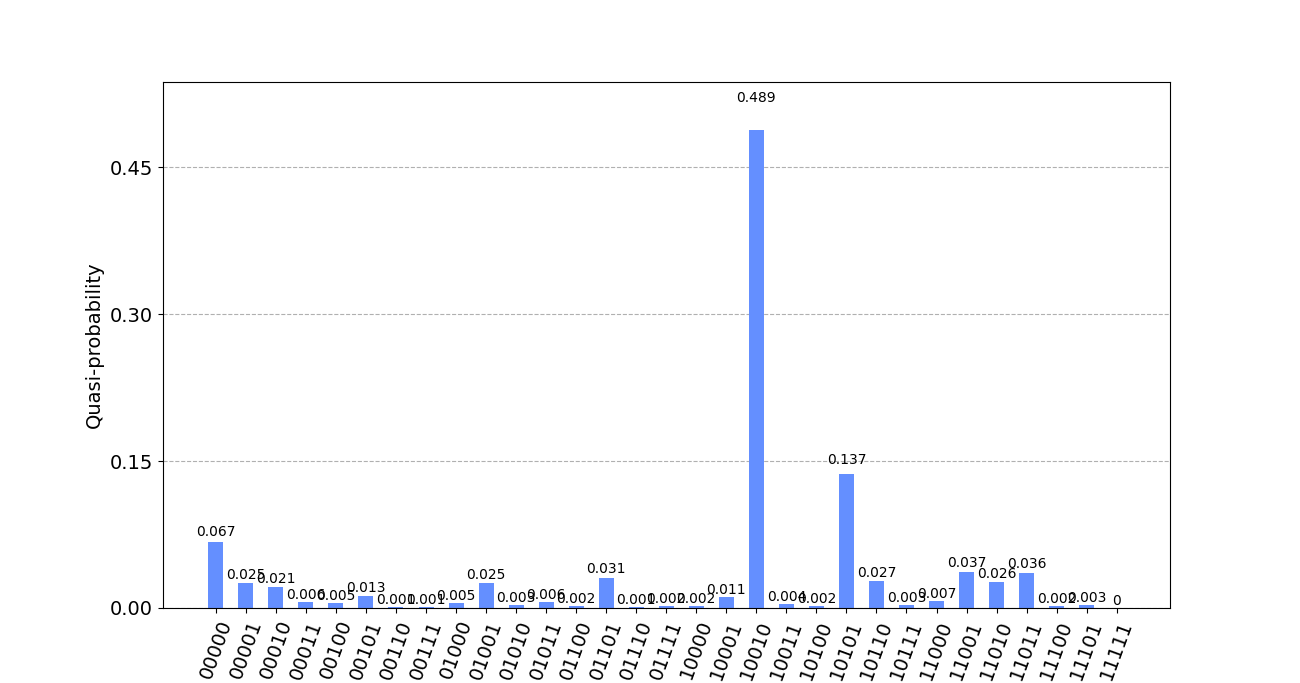
\includegraphics[width=0.47\textwidth]{caso_2_new}
  }
  \caption{Segundo caso}
\end{figure}

Al fin y al cabo se está computando el valor de la función de coste para todos los valores resultantes. Esto no es necesariamente costoso computacionalmente, ya que no se hace sobre todo el espacio de resultados posibles, sino sobre el resultante. Esta operación ya se hace para cada ejecución de la función \textit{execute\_circuit} en el optimizador COBYLA, así que otra vez no causa una diferencia.

De todas formas, como ya se obtiene el valor de la función de coste directamente se puede obtener la cadena de bits con menor coste y ya está el mejor resultado obtenido en el diccionario. Esto debe ser lo que se hace en D-Wave, ya que al obtener el resultado de una ejecución se muestran las cadenas de bits y al lado la energía asociada.

\end{document}

%%% Local Variables:
%%% mode: latex
%%% TeX-master: t
%%% End:
